\section{System Overview}

\begin{figure*}[htbp]
\begin{center}
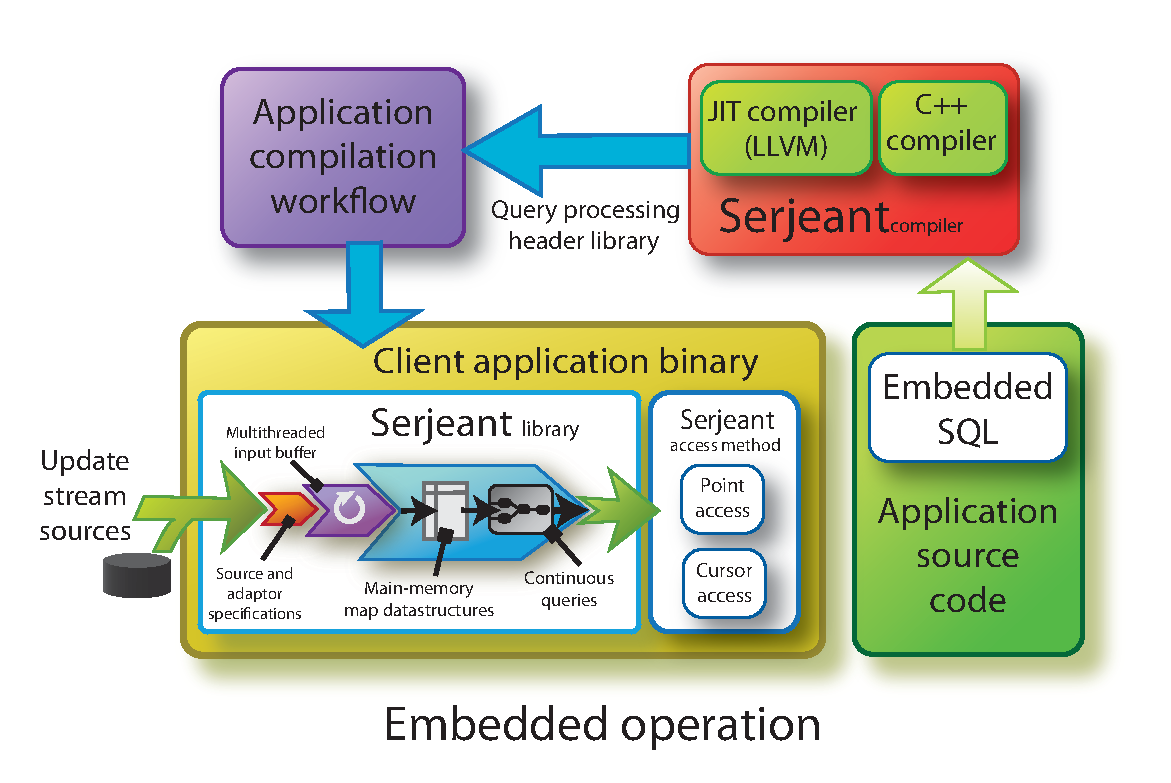
\includegraphics[scale=0.4]{figures/dbt-arch-embedded}
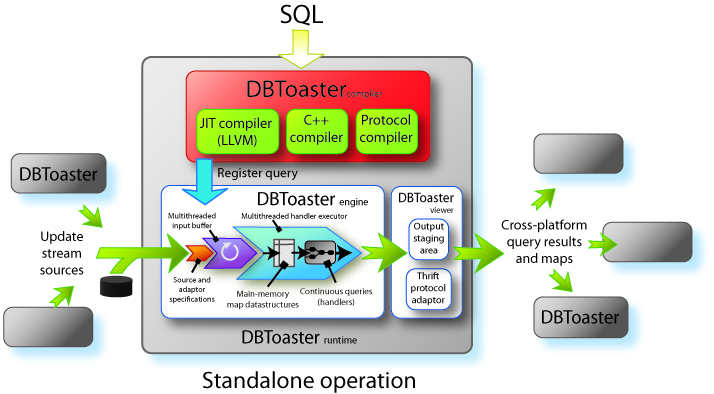
\includegraphics[scale=0.4]{figures/dbt-arch-standalone}
\end{center}
\caption{\compiler\ compiled query evaluation modes: i) compilation for embedded
  query processing ii) query object compilation for use in a distributed stream
  processing engine. \todo{Anonymize figures.}}
\label{fig:overview}
\end{figure*}

\compiler\ produces queries for use in two scenarios, first as an embedded query
processor that can be directly compiled into user applications, and second as a
query object that can be dynamically instantiated and executed in \compiler's
scalable, distributed, query execution infrastructure.

With embedded operation, \compiler's queries provide direct in-process query
processing functionality to client applications. By running in the same process
space, queries are able to provide extremely efficient access to query results,
and the contents on internal maps computed by \compiler. These maps can be used
in answering other queries, for example, queries with differing group-by fields
as often performed in datacube applications.
In this mode, \compiler behaves as a preprocessor in the application's build
workflow, generating a C++ header library that can be included where needed.
The C++ code produced by \compiler\ provides two access methods for pull-based
retrieval of query results beyond scalar aggregate results, first point access
(i.e. key lookups) to maps, and second a cursor-like read-only iteration over
maps. The cursor-oriented interface uses a private memory segment to provide
snapshot views of maps to applications, while \compiler's internal maps are
continuously updated with tuples arriving on streams.
Figure~\ref{fig:overview}i. shows an architecture diagram of \compiler\ and its
queries in the context of embedded processing.

For scalable query processing, we are currently developing a distributed stream
proessing infrastructure capable of compiling and executing source code produced
by \compiler\ in a dynamic on-demand fashion. Our approach is to use
just-in-time compilation to build query micro-engines, basing our system on the
Low-Level Virtual Machine (LLVM) framework as the JIT compiler for C++. The
compiled queries support both push- and pull-based query result and map
retrieval, with pull-based access to maps being similar to the cursor interface
described above for embedded operation. The \compiler\ compiler also includes an
additional code generation component to build a network protocol on top of
Apache Thrift to provide a simple and efficient binary protocol for results and
maps. Current topics include exploiting compilation to enable and enhance the
parallelism present in queries, including using static analysis techniques to
perform partitioning and allocating maps to different nodes in the distributed
system. Figure~\ref{fig:overview}ii. shows an architecture diagram of the
scalable query evaluation infrastructure.